\documentclass[]{scrreprt}
\usepackage{amsmath,graphicx}
\usepackage{multirow}
\usepackage{pslatex}
\usepackage{tabularx}
\usepackage{comment}
\usepackage{xspace}
\usepackage{array}

\usepackage{hyperref}

\usepackage{caption}
\DeclareCaptionFont{white}{\color{white}}
\DeclareCaptionFormat{listing}{\colorbox{gray}{\parbox{\textwidth}{#1#2#3}}}

\graphicspath{
{figures/}
}

\newcommand{\uo}{\mbox{UO\textsubscript{2}}\xspace}

\setcounter{secnumdepth}{3}

\newcommand{\si}{\sigma}
\newcommand{\mand}{\ \ \ \mbox{and}\ \ \ }
\newcommand{\pl}{\partial}
\newcommand{\ha}{\mbox{$\frac{1}{2}$}}
\newcommand{\thetac}{\theta^{\mathrm{c}}}
\newcommand{\thetarel}{\theta^{\mathrm{rel}}}
\newcommand{\ep}{\epsilon}
\newcommand{\ga}{\gamma}
\newcommand{\spa}{\ \ \ }
\newcommand{\non}{\nonumber}
\newcommand{\de}{\delta}
\newcommand{\ka}{\kappa}
\newcommand{\la}{\lambda}
\newcommand{\tr}{\mbox{Tr}\,}
\newcommand{\al}{\alpha}
\newcommand{\be}{\beta}
\newcommand{\cd}{\cdot}

\begin{document}


\title{Tensile Plasticity}
\author{CSIRO}
\maketitle

\tableofcontents


\chapter{Introduction and the yield functions}
\label{yf.chap}

Tensile, or Rankine, plasticity is designed to simulate a material
that fails when the maximum principal stress exceeds the material's tensile
  strength.  Its yield function is therefore
\begin{equation}
  f =  \sigma_{III} - T \ ,
\end{equation}
where $\sigma_{III}$ is the maximum\footnote{Often the maximum
  principal is denoted by $\sigma_{I}$, but the notation used in this
  document is motivated by the C++ code.  The code uses the {\tt
    dsymmetricEigenvalues} method of {\tt RankTwoTensor} and this
  orders the eigenvalues from smallest to greatest.} principal
stress (the largest eigenvalue of the stress tensor) and $T$ is the
tensile strength.

One yield function is sufficient because of the definition
$\sigma_{I}\leq\sigma_{II}\leq\sigma_{III}$.  For instance, if during
the return-map process both $\sigma_{II}$ and $\sigma_{III}$ exceed
$T$ the corresponding admissible configuration is that both of them
are equal to $T$.  While one yield function is sufficient, it is
convenient to use three yield functions in total:
\begin{eqnarray}
  f_{0} & = & \sigma_{III} - T \ , \nonumber \\
  f_{1} & = & \sigma_{II} - T \ , \nonumber \\
  f_{2} & = & \sigma_{I} - T \ .
  \label{yfs}
\end{eqnarray}
This is the version used by {\tt TensileStressUpdate}.

The return-map algorithm first rotates $\sigma$ from the physical
frame to the
principal-stress frame (where $\sigma = \mbox{diag}(\sigma_{I}, \sigma_{II},
\sigma_{III})$).  The rotation matrices used are assumed not to change
during the return-map process: only $\sigma_{I}$, $\sigma_{II}$ and
$\sigma_{III}$ change.  Therefore, at the end of the
return-map process these rotation matrices may be used to find the
final stress in the physical frame.

The three yield functions of Eqn~(\ref{yfs}) are smoothed using the
method encoded in {\tt MultiParameterPlasticityStressUpdate}.  An
example is shown Figures~\ref{tensile_3D.fig}
and~\ref{tensile_oct.fig}.  Figure~\ref{tensile_oct.fig} shows slices
of the yield surface at three values of the mean stress, and the
triangular-pyramid nature of the yield surface is evident.  The slices
are taken near the tip region only, to highlight: (1) the smoothing;
(2) that the smoothing is unsymmetric.

The unsymmetric nature of the
yield surface only occurs near the tip region where the smoothing
mixes the three yield surfaces.  For instance, the black line in
Figure~\ref{tensile_oct.fig} is symmetric, while the blue and red
lines are unsymmetric.  The amount of asymmetry is small, but it is
evident that the red curve is not concentric with the remainder of the
curves shown in Figure~\ref{tensile_oct.fig}.  The order of the yield
functions in Eqn~(\ref{yfs}) has been chosen so that the curves
intersect the $\sigma_{III}=\sigma_{II}$ line at $90^{\circ}$, but not
on the $\sigma_{II}=\sigma_{I}$ line near the pyramid's tip.  The
asymmetry does not affect MOOSE's convergence, and of course it is
physically irrelevant (since there is no one ``correct'' smoothed
yield surface).

\begin{figure}[htb]
  \begin{center}
    \begin{tabular}{ll}
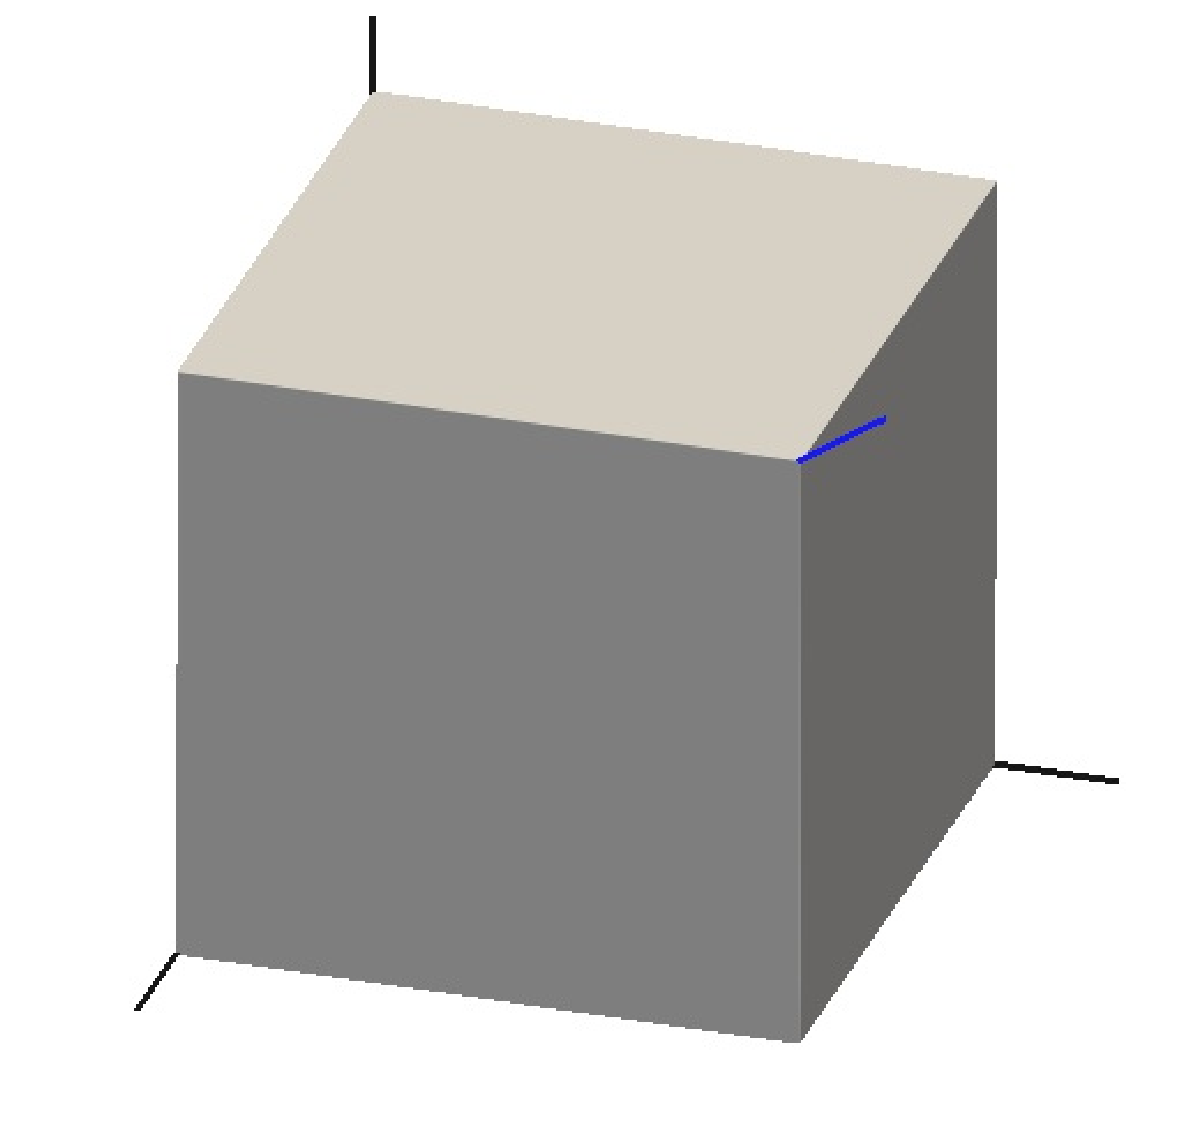
\includegraphics[width=6cm]{../../../../large_media/solid_mechanics/theory/tensile_unsmoothed.eps} &
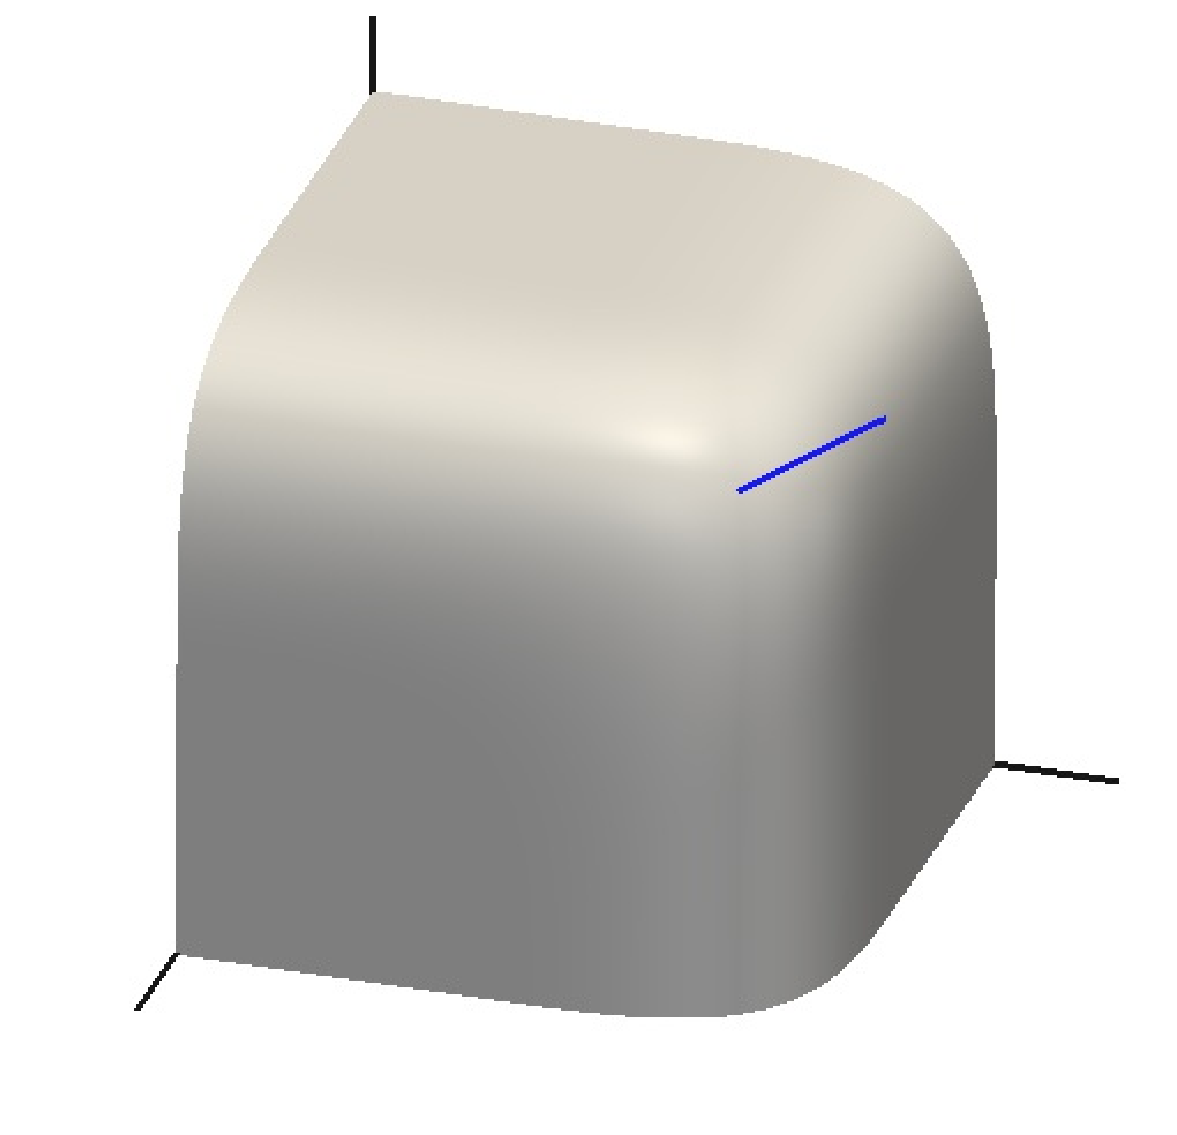
\includegraphics[width=6cm]{../../../../large_media/solid_mechanics/theory/tensile_smoothed.eps}
    \end{tabular}
\caption{Left: the unsmoothed yield surface defined by
  Eqn~(\ref{yfs}) is a trianglar pyramid.  Right: a smoothed version.  The principal stress
  directions are shown with black lines, and the mean stress direction
  is shown with a blue line.  The three planes extend infinitely
  (there is no base to the triangular pyramid) but these pictures show
  the tip region only.}
\label{tensile_3D.fig}
\end{center}
\end{figure}

\begin{figure}[htb]
  \begin{center}
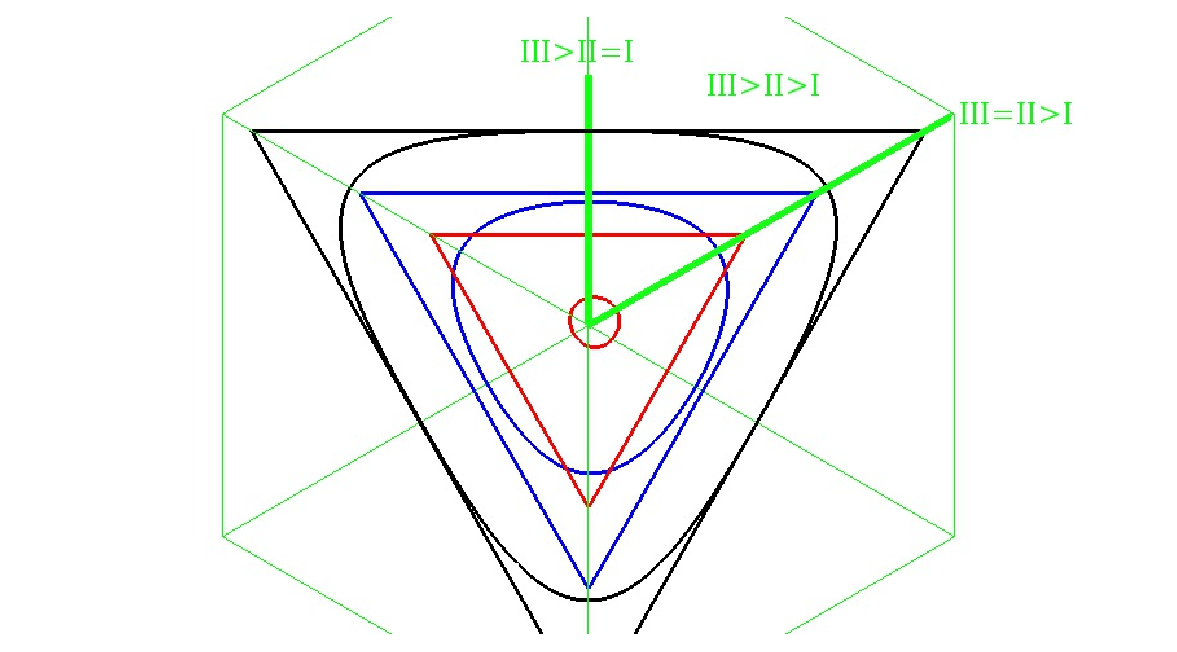
\includegraphics[width=10cm]{../../../../large_media/solid_mechanics/theory/octahedral_plane_tensile.eps}
\caption{Slices of the unsmoothed and smoothed yield functions at
  various value of mean stress.  In this example $T=1$, the smoothing
  tolerance is 0.5, and the values of mean stress shown are: black,
  0.7; blue, 0.8, red 0.85.  An unusually large amount of smoothing
  has been used here to highlight various features: in real
  simulations users are encouraged to use smoothing approximately
  $T/10$.  The whole octahedral plane is shown in this figure, but
  only one sextant is physical, which is indicated by the solid green
  lines.}
\label{tensile_oct.fig}
\end{center}
\end{figure}


\chapter{Flow rules and hardening}

This plasticity is associative: the flow potential is
\begin{equation}
  g = f = max(f_{0}, f_{1}, f_{2}) + \mbox{smoothing} \ .
\end{equation}
Here ``smoothing'' indicates the smoothing mentioned in
Chapter~\ref{yf.chap}.

The flow rules are
\begin{equation}
  s_{a} = s_{a}^{\mathrm{trial}} - \ga E_{ab} \frac{\partial
    g}{\partial s_{a}} \ ,
  \label{eqn.flow.rules}
\end{equation}
where $s_{a}=\{\sigma_{I}, \sigma_{II}, \sigma_{III}\}$ and
\begin{equation}
  E_{ab} = \frac{\partial s_{a}}{\partial \sigma_{ij}} E_{ijkl}
  \frac{\partial s_{b}}{\partial \sigma_{kl}} \ .
\end{equation}
In this equation $E_{ijkl}$ is the elasticity tensor.

An assumption
that is made in {\tt  MultiParameterPlasticityStressUpdate} is that
$E_{ab}$ is independent of the stress parameters, $s_{a}$ and the
internal variables.  In this case\footnote{Special precautions are
  taken when the eigenvalues are equal, as described in {\tt RankTwoTensor}.}
\begin{equation}
  \frac{\partial s_{a}}{\partial \sigma_{ij}} = v_{i}^{a}v_{j}^{a} \ ,
\end{equation}
where $v^{a}$ is the eigenvector corresponding to the eigenvalue
$s^{a}$ (of the stress tensor) and there is no sum over $a$ on the
right-hand side.  Recall that the eigenvectors are fixed during the
return-map process, so the RHS is fixed, meaning that $E_{ab}$ is
indeed independent of the stress parameters.  Also recall that the
eigenvectors induce a rotation (to the principal-stress frame), so
assuming that $E_{ijkl}$ is isotropic
\begin{equation}
  E_{ab} = E_{aabb} \ .
\end{equation}
The assumption of isotropy is appropriate for this type of isotropic
plasticity.

It is assumed that there is just one internal parameter, $i$, and that
it is defined by
\begin{equation}
  i = i_{\mathrm{old}} + (\sigma_{III}^{\mathrm{trial}} - \sigma_{III})
  / E_{22} \ ,
\end{equation}
during the return-map process.  The tensile strength is a function of
this single internal parameter

\chapter{Technical discussions}

\section{Unknowns and the convergence criterion}
The return-map problem involves solving the four equations: $f=0$ (smoothed yield function
should be zero) and the flow equations~(\ref{eqn.flow.rules}).  The
unknowns are the 3 stress parameters $s_{a}=\{\sigma_{I}, \sigma_{II},
\sigma_{III}\}$ and the plasticity multiplier $\ga$.  Actually, to
make the units consistent the algorithm uses $\ga E_{22}$ instead of
simply $\ga$.  Convergence
is deemed to be achieved when the sum of squares of the residuals of
these 4 equations is less than a user-defined tolerance.

\section{Iterative procedure and initial guesses}
A Newton-Raphson process is used, along with a cubic line-search.  The
process may be initialised with the solution that is correct for
perfect plasticity (no hardening) and no smoothing, if the user
desires.  Smoothing adds nonlinearities, so this initial guess will
not always be the exact answer. For hardening, it is not
always advantageous to initialise the Newton-Raphson process in this
way, as the yield surfaces can move dramatically during the return
process.

\section{Substepping the strain increments}
Because of the difficulties encountered during the Newton-Raphson
process during rapidly hardening/softening moduli, it is possible to
subdivide the applied strain increment, $\delta\epsilon$, into smaller
substeps, and do multiple return-map processes.  The final returned configuration may then
be dependent on the number of substeps.  While this is simply
illustrating the non-uniqueness of plasticity problems, in my
experience it does adversely affect MOOSE's nonlinear convergence as
some Residual calculations will take more substeps than other Residual
calculations: in effect this is reducing the accuracy of the Jacobian.

\section{The consistent tangent operator}
MOOSE's Jacobian depends on the derivative
\begin{equation}
H_{ijkl} = \frac{\delta\sigma_{ij}}{\delta \epsilon_{kl}} \ .
\end{equation}
The quantity $H$ is called the consistent tangent operator.  For pure
elasticity it is simply the elastic tensor, $E$, but it is more
complicated for plasticity.  Note that a small $\delta\epsilon_{kl}$
simply changes $\delta\sigma^{\mathrm{trial}}$, so $H$ is capturing the
change of the returned stress ($\delta\sigma$) with respect to a
change in the trial stress ($\delta\sigma^{\mathrm{trial}}$).  In formulae:
\begin{equation}
  H_{ijkl} = \frac{\delta\sigma_{ij}}{\delta
    \sigma_{mn}^{\mathrm{trial}}}
  \frac{\delta\sigma_{mn}^{\mathrm{trial}}}{\delta\epsilon_{kl}} =\frac{\delta\sigma_{ij}}{\delta
    \sigma_{mn}^{\mathrm{trial}}} E_{mnkl} \ .
\end{equation}

In the case at hand,
\begin{equation}
  \sigma_{ij} = \sum_{a}R_{ia}s_{a}R_{aj}^{\mathrm{T}} \ .
\end{equation}
In this formula $\sigma_{ij}$ is the returned stress, $s_{a}$ are the
returned stress parameters (eigenvalues), and $R$ is the rotation
matrix, defined through the eigenvectors, $v^{a}$ ($a=1,2,3$) of the
trial stress:
\begin{equation}
  R_{ia} = v^{a}_{i} \ .
\end{equation}
The three eigenvectors remain unchanged during the return-map
process.  However, of course they change under a change in
$\sigma^{\mathrm{trial}}$.  The relevant formulae are
\begin{eqnarray}
  \frac{\delta s_{a}^{\mathrm{trial}}}{\delta
    \sigma_{kl}^{\mathrm{trial}}} & = & v^{a}_{i}v^{a}_{j} \ , \\
  \frac{\delta v^{a}_{i}}{\delta \sigma_{kl}^{\mathrm{trial}}} & = &
  \sum_{b\neq a}\frac{v_{i}^{b}(v_{k}^{b}v_{l}^{a} +
    v_{l}^{b}v_{k}^{a})}{2(s_{a}-s_{b})} \ .
\end{eqnarray}
On the RHS of these equations there is no sum over $a$.

The final piece of information is
\begin{equation}
  \frac{\delta s_{b}}{\delta s_{a}^{\mathrm{trial}}} \ .
\end{equation}
{\tt MultiParameterPlasticityStressUpdate} computes this after each
Newton step, for any aribtrary plasticity model.

The nontrivial part to the consistent tangent operator is therefore
\begin{equation}
  \frac{\delta \sigma_{ij}}{\delta\sigma_{mn}^{\mathrm{trial}}} =
\sum_{a}  \frac{\delta
    R_{ia}}{\delta\sigma_{mn}^{\mathrm{trial}}}s_{a}R_{aj}^{\mathrm{T}}
  + \sum_{a}\sum_{b} R_{ia}\frac{\delta s_{a}}{\delta s_{b}^{\mathrm{trial}}}
  \frac{\delta s_{b}^{\mathrm{trial}}}{\delta
    \sigma_{mn}^{\mathrm{trial}}}R_{aj}^{\mathrm{T}} +
  \sum_{a} R_{ia}s_{a}\frac{\delta
    R_{aj}^{\mathrm{T}}}{\delta\sigma_{mn}^{\mathrm{trial}}} \ .
\end{equation}
All the components of this equation have been provided above.


\end{document}

